\documentclass[paper=a4, twoside, fontsize=12pt, parskip=half-, numbers=enddot, open=right]{scrbook}
\usepackage{preambule}
\usepackage{macros}
\begin{document}

\chapter*{Rappels de géométrie}
\section{Vocabulaire et notations}

Trace \(AD\) en rouge, \(\lbrack CD\rbrack\) en vert, \(AB\rbrack\) en gris, \(\lbrack BC\rbrack\) en noir et \(\lbrack EC\) en bleu. \\ Nomme \(X\) l'intersection entre \(AD\) et \(\lbrack EC\).

\begin{center}
    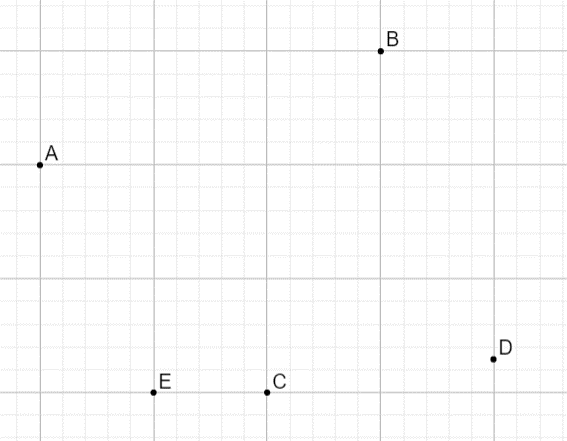
\includegraphics[width=.5\linewidth]{img/intro.png}
\end{center}
Complète~:
\begin{enumerate}[itemsep=.7cm]
    \item \(AD\) représente \dotfill
    \item \(\lbrack CD\rbrack\) représente \dotfill
    \item \(AB\rbrack\) représente \dotfill
    \item \(\lbrack EC\ \) représente \dotfill
    \item \(X\) est un point de \(AD\). On dit que \(X\) \dotfill à \(AD\). Cela se note\(X\)\ldots \(AD.\)
    \item \(X\) n'est pas un point de \(AB\rbrack\). On dit que \(X\) \dotfill à \(AB\rbrack\). \\ Cela se note X \ldots \(AB]\).
\end{enumerate}

\newpage
\subsubsection{Un point}
Un point se note à l'aide d'une lettre majuscule. \\
Exemple :
\vspace{2cm}

\subsubsection{Une droite}
Une droite se note à l'aide soit d'une lettre minuscule, soit de deux lettres majuscules. Dans ce cas-là, nous nommons la droite par deux points de passage de cette droite. Une droite est illimitée. \\
Exemple :
\vspace{2cm}

\subsubsection{Une demi-droite}
Une demi-droite se note à l'aide de deux lettres majuscules. Nous nommons alors la demi-droite à l'aide de son origine (marquée d'un crochet) et d'un point de passage de cette demi-droite. \\
Exemple :
\vspace{2cm}

\subsubsection{Un segment de droite}
Un segment de droite se note à l'aide de deux lettres majuscules. Nous nommons le segment à l'aide des deux extrémités du segment, marquées par des crochets. \\
Exemple :
\vspace{2cm}

La longueur du segment se note :

\subsubsection{Droites parallèles}
Deux droites parallèles sont des droites qui soit n'ont aucun point commun, autrement dit qui n'auront aucun point d'intersection, soit qui sont confondues (donc elles possèdent une infinité de points d'intersections). Cela se note à l'aide du symbole \ldots .\\
Exemple :
\vspace{2cm}

\subsubsection{Droites sécantes}
Deux droites sécantes sont des droites qui ont un point commun, autrement dit qui ont un point d'intersection. Si deux droites ne sont pas parallèles, alors elles sont sécantes. Cela se note à l'aide du symbole \ldots .\\
Exemple :
\vspace{2cm}

\subsubsection{Droites perpendiculaires}
Deux droites perpendiculaires sont deux droites sécantes qui se coupent en formant quatre angles droits (=90° ). Cela se note à l'aide du symbole \ldots . \\
Exemple :
\vspace{2cm}

\subsubsection{Notion d'appartenance}
Un point appartient à une droite (ou à un segment, à une demi-droite, \ldots) s'il fait partie de cette droite. Cela se note à l'aide des symboles $\in$ (appartient à) et $\notin$ (n'appartient pas à).  \\
Exemple :
\vspace{2cm}

\newpage
\begin{exercise}
    Complète les pointillés à l'aide des symboles \(\in\) et \(\notin\).
    \begin{center}
        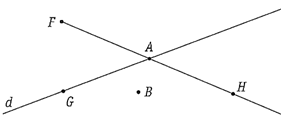
\includegraphics[]{img/appartient.png}
    \end{center}
    \begin{enumerate}[itemsep=1cm, cols=4]
        \item \(F \dotfill [AH\)
        \item \(B \dotfill d\)
        \item \(G \dotfill AG\)
        \item \(H \dotfill [FA\)
        \item \(A \dotfill d\)
        \item \(H \dotfill [AF\)
        \item \(G \dotfill d\)
        \item \(H \dotfill [AH]\)
    \end{enumerate}
    %\TODO: nouveau schéma 
\end{exercise}

\begin{exercise}
    Complète les pointillés à l'aide du symbole adéquat concernant la position relative de deux droites.
    \begin{multicols}{3}
        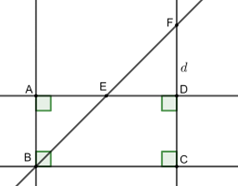
\includegraphics[]{img/pos_de_droites.png}

        \begin{enumerate}[itemsep=1cm]
            \item \(d \dotfill AB\)
            \item \(BF \dotfill d\)
            \item \(AB \dotfill CD\)
            \item \(AD] \dotfill CD\)
            \item \(BE \dotfill BC\)
            \item \(AD \dotfill d\)
            \item \(FC \dotfill AB\)
            \item \(EF \dotfill BC\)
        \end{enumerate}
    \end{multicols}
\end{exercise}

\begin{exercise}
    Construis la droite demandée.
    \tcbsidebyside[blanker]{
        Construis $d$ tel que $d \bot a$ et $C \in d$
        \bigbreak
        \includegraphics{tikz/droite_construction.tikz}
    }{
        Construis $f$ tel que $f \sslash AB$ et $C \notin f$
        \bigbreak
        \includegraphics{tikz/droite_construction.tikz}
    }
\end{exercise}

\newpage
\begin{exercise}
    Place trois points non alignés \(A,\ B\ C\). Trace les éléments suivants~:
    \begin{enumerate}
        \item \(AB\)
        \item \([BC\)
        \item \([AC]\)
        \item La droite \(d\) perpendiculaire à \(AB\) passant par \(A\)
        \item La droite \(d'\) parallèle à \(AB\) passant par \(C\)
    \end{enumerate}
\end{exercise}

\vfil

\begin{exercise}
    Construis une demi-droite que tu nommes \(\lbrack AC\). \\
    Trace \(e\), parallèle à \(\lbrack AC\) à \(2cm\) de \(\lbrack AC\). \\
    Place \(F\), tel que \(F \in \lbrack AC\ \)et \(|AF| = 1,5\ cm\)
\end{exercise}

\newpage
\section{La médiatrice}

\dotsforanswer{3}[La médiatrice d'un segment est]

\begin{enumerate}[itemsep=2cm, cols=2, label= ]
    \item Tracé à l'équerre :
    \item 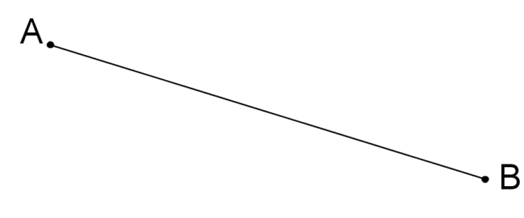
\includegraphics[]{img/segmentAB.png}
    \item Tracé au compas :
    \item 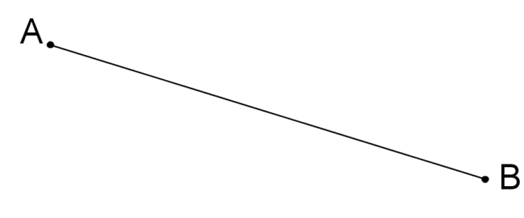
\includegraphics[]{img/segmentAB.png}
\end{enumerate}

\vfil

\begin{exercise}
    Maxime a tracé trois médiatrices. Laquelle est correcte~? Explique pourquoi les deux autres ne le sont pas.
    \begin{center}
        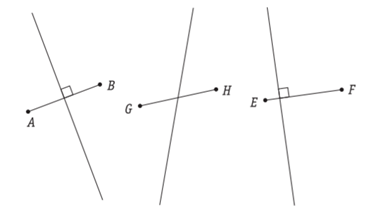
\includegraphics[]{img/med.png}
    \end{center}
    \dotsforanswer{3}[]
\end{exercise}

\newpage
\section{Les angles}
Un angle est une partie du plan délimitée par deux demi-droites de même origine. Ces deux demi-droites sont les côtés de l'angle et l'origine est le sommet de cet angle.\\
Exemple~:
\vspace{3cm}

L'angle peut s'écrire de différentes façons : \dotfill \\

L'amplitude de l'angle se mesure en degrés et s'écrit \dotfill
\subsubsection{Types d'angles}
%Synthèse des différents angles (aigus, obtus, droits, plein, plat, nul)

\newpage
\begin{exercise}
    Après avoir été programmé, un robot se déplace de la manière suivante~:
    \begin{multicols}{2}
        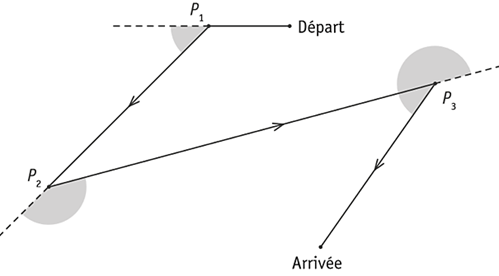
\includegraphics[]{img/robot.png}
        À l'aide des instruments adéquats, mesure l'amplitude des angles grisés.
        \begin{enumerate}[itemsep=1cm, label= ]
            \item \(|\widehat{P_1}| =\)
            \item \(|\widehat{P_2}| =\)
            \item \(|\widehat{P_3}| =\)
        \end{enumerate}
    \end{multicols}
\end{exercise}

\begin{exercise}
    Trace les angles dont les amplitudes sont données ci-dessous.
    \begin{enumerate}[cols=2, itemsep=6cm, label= ]
        \item \(|\widehat{O}|=111\degres\)
        \item \(|\widehat{B}|=50\degres\)
        \item \(|\widehat{BAC}|=62\degres\)
        \item \(|\widehat{SPI}|=250\degres\)
    \end{enumerate}
    \vspace{6cm}
\end{exercise}

\newpage
\section{La bissectrice}

\dotsforanswer{4}[La bissectrice d'un angle est]

\begin{enumerate}[itemsep=3cm, cols=2, label= ]
    \item Tracé à l'équerre :
    \item 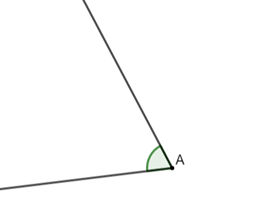
\includegraphics[]{img/angleA.png}
    \item Tracé au compas :
    \item 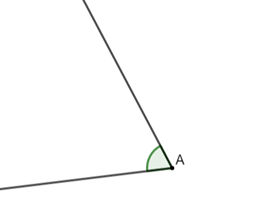
\includegraphics[]{img/angleA.png}
\end{enumerate}

\begin{exercise}
    Trace un angle \(\widehat{POM}\) tel que \(|\widehat{POM}|=150\degres\). \\
    Trace au compas la bissectrice (\(b\)) de cet angle. \\
    Place le point \(K \in b\) tel que \(\overline{KO}=2cm\). \\
    Trace \(a\), perpendiculaire à \([OP\) passant par \(K\).
\end{exercise}

\newpage
\section{Exercices mélangés}
\setcounter{exercise}{0}

\begin{exercise}
    Décode les notations géométriques suivantes.
    \begin{enumerate}[cols=4]
        \item \(\lbrack CD\)
        \item \(D\)
        \item \(\widehat{SEV}\)
        \item \(F\  \in \lbrack BV\rbrack\)
        \item \(\overline{CD}\)
        \item \(MN\  \nparallel BC\)
        \item \(|\widehat{PME}|=80\degres\)
        \item \(S\  \in RI\)
        \item \(CD\rbrack\)
        \item \(|CD|\)
        \item \(M\  \notin m\)
        \item \(d \bot p\)
    \end{enumerate}
\end{exercise}

\begin{exercise}
    Vrai ou faux? Lorsque c'est faux, justifie ou donne un contre-exemple.
    \begin{enumerate}
        \item Un angle aigu a toujours une amplitude plus petite que celle d'un angle plat.
        \item Un angle plein est un angle nul.
        \item La somme de deux angles aigus donne toujours un angle obtus.
        \item Si on additionne l'amplitude d'un angle aigu à celle d'un angle obtus, on obtient toujours un angle plat.
    \end{enumerate}
\end{exercise}

\begin{exercise}

    \begin{enumerate}[label= $\ast $]
        \item Trace une droite $f$.
        \item Place un point $R$ tel que $R \notin f$.
        \item Trace $a$ tel que $a \parallel f$.
        \item Trace $CD$ tel que $CD \parallel a \parallel f$.
        \item Trace $[RD]$
    \end{enumerate}
\end{exercise}

\begin{exercise}
    Place trois points non alignés que tu appelleras $R$, $A$ et $Y$.
    \begin{enumerate}[label= $\ast$]
        \item Trace $AR$ en vert
        \item Trace $RY]$ en bleu
        \item Trace $a$, parallèle à $AR$ et passant par $Y$.
        \item Trace $d$, perpendiculaire à $RY]$ ne passant pas par $A$
    \end{enumerate}
\end{exercise}

\begin{exercise}
    Trace un segment \([AB]\) qui mesurera \SI{5,5}{cm}. Trace ensuite, au compas, sa médiatrice.
\end{exercise}

\begin{exercise}
    Trace les angles demandés ainsi que leurs bissectrices (au compas).
    \begin{enumerate}[cols=2]
        \item \(|\widehat{LUI}|=260\degres\)
        \item \(|\widehat{MOI}|=75\degres\)
        \item \(|\widehat{EUX}|=11\degres\)
        \item \(|\widehat{TOI}|=195\degres\)
    \end{enumerate}
\end{exercise}

\end{document}
